\documentclass{beamer}
\usetheme{PegasusUCF}
\usepackage{hyperref}
\usepackage{graphicx}
\usepackage{tikz}
\usepackage{tkz-euclide}



%-------------------------------
\title[Math Review Slides]{Math Review Slides}
\author{Joshua L. Eubanks}

\newcommand{\deptname}{12}%ECONOMICS

%<<<<<
\date{\vspace{-8cm}}

%--------------------------------



%%%%%%%%%%%%%%%%
\begin{document}
%%%%%%%%%%%%%%%
\begin{frame}
  \titlepage
\end{frame}

\begin{frame}{Overview}
\tableofcontents
\end{frame}

\section{Calculating Area}

\begin{frame}{Calculating Area}

In this course, you will need to know how to calculate the area of a rectangle/square and the area of a triangle.

\end{frame}

\subsection{Area of Rectangle/Square}
\begin{frame}{Area of Rectangle/Square} 

  \begin{block}{Rectangle}
  A four-sided figure that has two sets of parallel sides, so that we have two sides of one length and two sides of another length.
  \end{block}

  \begin{block}{Square}
    A special case of a rectangle in which all four sides are the same length.
  \end{block}

Since the square is just a special case, the way to calculate the area is the same no matter whether we are dealing with a rectangle or a square.

\end{frame}

\begin{frame}{Area of Rectangle/Square Cont.}
  
  \begin{block}{Area of a Rectangle/Square Formula}
    $$Area = base \times height = b \times h$$

  \end{block}


In this formula, \textbf{the base is the width of the rectangle} and the \textbf{height is simply how tall the rectangle is}.

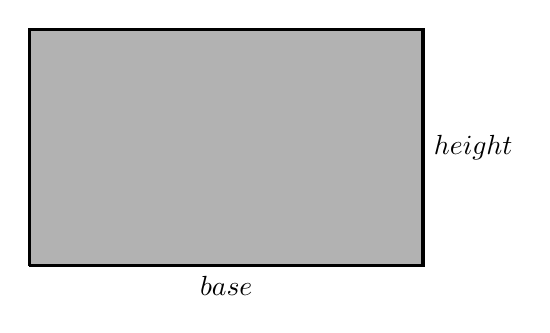
\begin{tikzpicture}
\filldraw[color=black, fill=black!30, very thick] (0,0)  -| (5,3) 
    node[pos=0.25,below] {$base$} 
    node[pos=0.75,right] {$height$}
    -| (0,0);
\end{tikzpicture}

\end{frame}

\begin{frame}{Area of Rectangle/Square Example}
  
  \begin{exampleblock}{Lot Size Example}
    Suppose you are looking at a house and the realtor says that it is a 300 foot by 150 foot plot of land. Calculate the square footage of the lot.
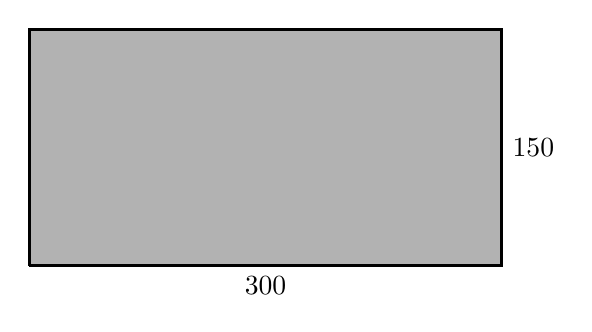
\begin{tikzpicture}
\filldraw[color=black, fill=black!30, very thick] (0,0)  -| (6,3) 
    node[pos=0.25,below] {$300$} 
    node[pos=0.75,right] {$150$}
    -| (0,0);
\end{tikzpicture}

$Area = base \times height = 300 \times 150 = 45$ thousand square feet

  \end{exampleblock}


\end{frame}


\subsection{Area of a Triangle}

\begin{frame}
 
  \begin{block}{Triangle}
  Essentially a rectangle cut in half. So the formula is half that of the rectangle.

  $$Area = \frac{1}{2} \times base \times height = \frac{1}{2} \times b \times h$$
  \end{block}

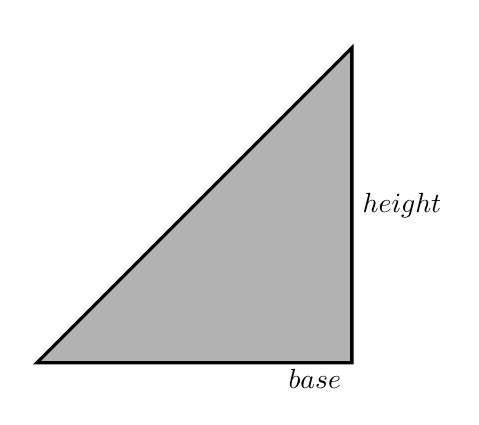
\begin{tikzpicture}
\filldraw[color=black, fill=black!30, very thick] (0,0) node[anchor=north]{$  $}
  -- (4,0) node[anchor=north]{$$}
  -- (4,4) node[anchor=south]{$$}
     node[pos= -0.05,anchor = east] {$base$} 
    node[pos=0.5,right] {$height$}
  -- cycle;
\end{tikzpicture}

\end{frame}

\section{Fractions}

\begin{frame}{Fractions}

  \begin{block}{Fraction}
  A fraction is just a proportion, consisting of a numerator and a denominator as follows:
 $$\frac{Numerator}{Denominator}$$
  \end{block}

We can add, subtract, multiply, or divide fractions.

\end{frame}

\subsection{Multiplying and Dividing Fractions}

\begin{frame}{Multiplying and Dividing Fractions}

\begin{block}{Multiplication}
We merely multiply the numerators and the denominators together to get the result
\end{block}

  \begin{exampleblock}{Multiplication Example}
  $$\frac{5}{7}\times \frac{2}{3} = \frac{5\times 2}{7\times 3} = \frac{10}{21}$$
  \end{exampleblock}
\end{frame}

\begin{frame}{Multiplying and Dividing Fractions Cont.}

\begin{block}{Division}
We simply \textit{invert} the second fraction by switching the numerator and the denominator. Then multiplying
\end{block}

  \begin{exampleblock}{Division Example}
  $$\frac{5}{7}\div \frac{2}{3} = \frac{5}{7}\times \frac{3}{2} = \frac{5\times 3}{7\times 2} = \frac{15}{14}$$
  \end{exampleblock}
\end{frame}

\subsection{Adding and Subtracting Fractions}


\begin{frame}{Adding and Subtracting Fractions}
  \begin{block}{Case 1: Denominators Match}
    t is simply a matter of adding or subtracting the numbers in the numerator and leaving the denominator as it is.
  \end{block}
  \begin{exampleblock}{Examples when Denominators Match}
  \begin{align}
    \frac{5}{12} + \frac{2}{12} &= \frac{7}{12}\\
    \frac{6}{7} - \frac{2}{7} &= \frac{4}{7}
  \end{align}
  \end{exampleblock}

\end{frame}

\begin{frame}{Adding and Subtracting Fractions Cont.}
  \begin{block}{Case 2: Denominators Do Not Match}
    \begin{itemize}
      \item You cannot simply repeat the process in case 1. We first need to convert the fractions to a common denominator.
      \item We can create a common denominator by multiplying top and bottom of the first fraction by the denominator of the second fraction and multiplying top and bottom of the second fraction by the denominator of the first.
    \end{itemize}

  \end{block}

  \begin{exampleblock}{Example when Denominators Do Not Match}
  $$\frac{3}{4}+ \frac{5}{3} = \frac{3}{3}\times \frac{3}{4} + \frac{4}{4} \times \frac{5}{3} = \frac{3\times 3}{3\times 4} + \frac{4\times 5}{4\times 3} = \frac{9}{12}+\frac{20}{12}= \frac{29}{12}$$
  \end{exampleblock}

\end{frame}

\section{Graphing}

\subsection{Cartesian Coordinate System}

\begin{frame}{Cartesian Coordinate System}

\begin{block}{Cartesian Coordinate System}

Two-dimensional graph that is the intersection of two perpendicular lines one of which is horizontal. The point of intersection is called the \textit{origin}
\end{block}
\begin{center}

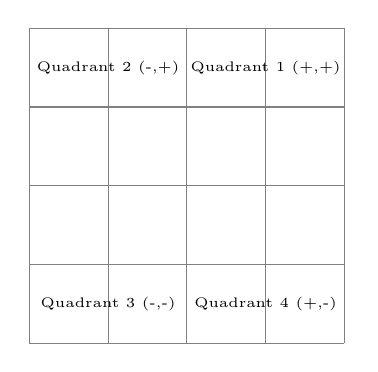
\begin{tikzpicture}
   \tkzInit[xmax=2,ymax=2,xmin=-2,ymin=-2]
   \tkzGrid
   \tkzAxeXY
 two points for drawing 2x+y=2
  \tkzText( 1,1.5){\tiny{Quadrant 1 (+,+)}}
  \tkzText(-1,1.5){\tiny{Quadrant 2 (-,+)}}
  \tkzText(-1,-1.5){\tiny{Quadrant 3 (-,-)}}
  \tkzText(1,-1.5){\tiny{Quadrant 4 (+,-)}}
  \end{tikzpicture}
\end{center}
\end{frame}

\subsection{Graphs}

\begin{frame}{Graphs}


  Most graphs in economics are based only Quadrant 1. We typically see only positive values for price, quantity, time, etc. There is one line called the \textbf{horizontal axis} and one called the \textbf{vertical axis}. They show the measurements of the $x$-variable and $y$-variable respectively

  \begin{block}{Horizontal Axis}
    Also known as the $x$-axis or abscissa, it is the solid horizontal line at the bottom of the graph. The values of the $x$-variable are measured along it.
  \end{block}

  \begin{block}{Vertical Axis}
    Also known as the $y$-axis or ordinate, it is the solid vertical line on the left-hand side of the graph -- remember, only looking at quadrant 1. The values of the $y$-variable are measured along it.
  \end{block}


\end{frame}

\begin{frame}{Graphs Cont.}

  \begin{block}{Origin}
    The point where the two axes meet, each variable is equal to zero. As you move rightward from the origin along the $x$-axis, values of the $x$-variable are positive and increasing. As you move up from the origin along the $y$-axis, values of the $y$-variable are
positive and increasing.
  \end{block}

\end{frame}


\begin{frame}{Graphing Example}
  \begin{exampleblock}{Ice Cream Sales}
    The table below shows the data on the outside temperature and the number of ice cream cones that a typical vendor can expect to sell at a football stadium during one game.

    \begin{tabular}{ c c c }\hline
Temperature & Ice Cream Sales & Point\\\hline
40 &  0 & A \\
60 & 10 & B \\
70 & 30 & C \\
80 & 50 & D \\
90 & 70 & E \\\hline
\end{tabular}
  \end{exampleblock}
\end{frame}

\begin{frame}

\begin{itemize}
  \item We typically put the \textit{dependent} variable on the $y$-axis. In this case ice cream sales depend on the weather outside.
  \item You can plot each of the five points A through E on the graph by using a pair of numbers: the values that the $x$-variable and the $y$-variable take on for a given point.
  \item For example, at point A, the $x$-variable takes on the value of 40 and the $y$-variable takes on the value of 0.
\end{itemize}

\begin{center}
\includegraphics[width = 0.6\textwidth]{IceCreamSales.png}
\end{center}
\end{frame}

\begin{frame}

\begin{itemize}
  \item When you connect points A, B, C, D, and E on the graph, such a line on a graph is called a curve, regardless of whether it is a straight line or a curved one. If the curve that shows relationship is a straight line, or \textbf{linear}, the variables have \textbf{linear relationship}. If the curve is not a straight line, or is \textbf{nonlinear}, the variables have a \textbf{nonlinear relationship}.

  \item The shape and the direction of the curve reveal the general nature of the relationship. When an increase in one variable is associated with an increase in the other variable, the two variables are said to have a \textbf{positive relationship}. When an increase in one variable is associated with a decrease in the other variable, the two variables are said to have a \textbf{negative relationship}. If two variables are independent of each other, then there is no relationship between two variables.

  \item In our Ice Cream example, there was a positive relationship between outside temperature and ice cream sales. As it gets hotter outside the amount of ice cream sold also increases.

\end{itemize}
  
\end{frame}

\section{Slope and Rate of Change}

\begin{frame}{Slope of a Linear Curve}

\begin{block}{Slope of a Line}
A measure of how sensitive the $y$-variable is to a change in the $x$-variable

$$Slope = \frac{\Delta y}{\Delta x} = \frac{y_{2}-y_{1}}{x_{2}-x_{1}}$$   
\end{block}

$\Delta$ (delta) is the greek symbol that means ``change in.'' When a variable increases, the change is positive; when a variable decreases, the change is negative.
\end{frame}

\begin{frame}{Slope of a Linear Curve Cont.}

\begin{block}{Case 1: Slope is Positive}
The rise (change in $y$) has the same sign (positive or negative) as the run (change in $x$).   
\end{block}

\begin{block}{Case 2: Slope is Negative}
when the rise and the run have opposite signs (one is positive and one is negative).   
\end{block}

\begin{block}{Case 3: Slope is 0}
When a curve is a straight horizontal line, the value of $y$ along the curve never changes or is constant. Therefore, everywhere along the curve, the change in $y$ is zero. So, regardless of the value of the change in $x$, the slope of a horizontal line is always zero.   
\end{block}

\end{frame}

\begin{frame}
\begin{block}{Case 4: Slope is $\infty$}
When a curve is a straight vertical line, the value of x along the curve never changes or is constant. Therefore, everywhere along the curve, the change in x is zero. It implies that the slope of a vertical line is a ratio with zero in the denominator. A ratio with zero in the denominator is equal to infinity
\end{block}
\end{frame}

\subsection{Percentages and Ratios}

\begin{frame}{Ratios and Percentages}
  \begin{block}{Ratios}
    Expressions of one value in terms of another. We can express these ratios in their fraction, decimal or percentage form.
  \end{block}

\begin{exampleblock}{Representing Number of Economics Majors in Class}
  Suppose we have 231 Economics majors in our class. The total number of students is 1192.\\

  \begin{itemize}
\item As a fraction $\frac{231}{1192}$

\item As a decimal, simply divide numerator by denominator: $\frac{231}{1192} \approx .1938$

\item As a percentage, take the decimal and multiply it by 100\%: $\frac{231}{1192}\times 100 \approx .1938\times 100 \approx 19.38\%$
\end{itemize}
\end{exampleblock}


\end{frame}

\subsection{Changes in Percentages}

\begin{frame}{Changes in Percentages}
\begin{itemize}
\item Suppose in our previous example, we get additional students that change their major to economics (now 331 instead of 231). How could we represent this change?  
\item  We begin by subtracting the former value from the latter value; in other words, if we call our first value $Q1$ and our second $Q2$, we want to calculate $Q2 – Q1$. In this example, $Q1$ is 231 and $Q2$ is 331. We can turn both of these numbers into fractions and then subtract the difference to come up with the percentage change.
\end{itemize}
\begin{alertblock}{Note}
In this example, the denominators are the same, so we can do this operation easily. If they did not match, we would have to match denominators first.
\end{alertblock}

\end{frame}


\begin{frame}

\begin{exampleblock}{Increase in Economics Majors}
Suppose the number of Econ majors increased to 331. What is the growth in economics majors?

$$\frac{Q2}{NumEnrolled} - \frac{Q1}{NumEnrolled} = \frac{331}{1192} - \frac{231}{1192}$$

Since the denominators are the same, we can simply subtract the numerators
$$\frac{331}{1192} - \frac{231}{1192} = \frac{100}{1192}$$
We could simply that fraction, represent it as a decimal, or show it as a percent.

$$\frac{100}{1192} \times 100 \approx 8.4\%$$

We can say that economics majors as a percentage of the overall class grew by 8.4\% 
\end{exampleblock}

\end{frame}

\begin{frame}{Expressing a Change in a Single Value in Percentage Terms}
  Often times we are interested in the percent change of one variable. For example, stocks are often reported as a percent change from the previous closing. There are many ways to calculate percent change, but in this course, you will use this formula

  \begin{block}{Percent Change}
    Let $Original$ be the first value, $New$ be the second value. Then our formula is:

    $$\frac{New-Original}{Original}$$

    If we want to represent this as a percentage, simply multiply by 100
  \end{block}

\end{frame}

\begin{frame}{Application of Percent Change Formula}
\begin{exampleblock}{Percent Change in Bitcoin}
  On November 10, 2021 one BTC was equal to 66,351.8 USD. When the slides were created, one BTC is equal to 24,490.06 USD. What is the percent change? 

  $$\frac{New-Original}{Original} = \frac{24,490.06-66,351.8}{66,351.8} \approx -63.09\%$$
\end{exampleblock}
\end{frame}


\section{Systems of Equations}

\begin{frame}{Systems of Equations}

In our course, we are only going to look at the intersection of two equations. If there are two equations, there must also be two unknown variables. 

\begin{exampleblock}{Example}
  Suppose we have two equations and two unknowns:
  \begin{align*}
    2x + 3y &= 12\\ 
    x+y &=5
  \end{align*}
  What values of $x$ and $y$ satisfy both equations?
\end{exampleblock}

\end{frame}

\begin{frame}{Graphical Solution to System of Equations}

We can see this graphically:
\begin{center}
\includegraphics[width = 0.5\textwidth]{SystemsOfEquations.png}
\end{center}

Where the two lines intersect, is the solution. $(x^{*},y^{*}) = (3,2)$
\end{frame}

\begin{frame}{Solution to System of Equations by Substitution}

You simply isolate one of the variables by itself, then you plug it into the other equation and solve for the other variable. Plug that value into the isolated variable equation and you will have the answer. I am going to isolate the second equation because it is easier. 

$$y=5-x$$
Plugging into equation 1:
\begin{align*}
2x + 3(5-x) &= 12\\
2x + 15-3x &= 12\\
-x &= -3\\
x &= 3
\end{align*}

We can plug that into our original equation $y = 5 - 3 = 2$. So the solution is (3,2).

\end{frame}
%%%%%%%%%%%%%%
\end{document}